
\parbox{\textwidth}{
  \renewcommand{\arraystretch}{1.3}
  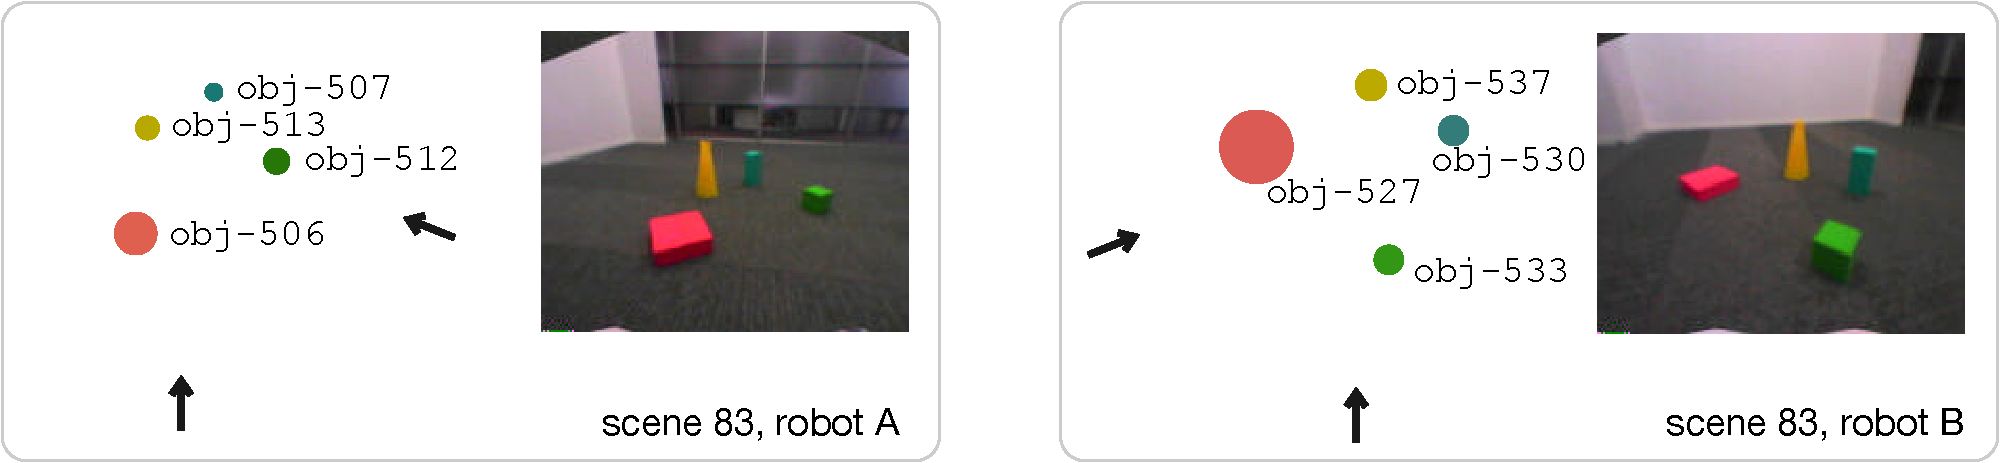
\includegraphics[width=1\textwidth]{figures/qfwm-example-world-models-scene-83}
  
  \vspace{0.5cm}
  \definecolor{dark}{rgb}{0.5,0.2,0}     
  \begin{tabular*}{\textwidth}{@{}p{2.05cm}@{}p{2.05cm}@{}p{2.05cm}@{}p{2.05cm}@{}||p{2.05cm}@{}p{2.05cm}@{}p{2.05cm}@{}p{2.05cm}}
    {\tt obj-512} & {\tt obj-507} & {\tt obj-513} & {\tt obj-506} & {\tt obj-533} & {\tt obj-530} & {\tt obj-537} & {\tt obj-527} \\
    \hline
    \textcolor{dark}{\slshape x-3 } & { x-4 } & { x-4} & \textcolor{dark}{\slshape  x-2} & \textcolor{dark}{\slshape  x-2} & {  x-4} & {  x-4} & \textcolor{dark}{\slshape  x-3} \\
    \textcolor{dark}{\slshape y-1} & \textcolor{dark}{\slshape y-2} & \textcolor{dark}{\slshape y-3} & \textcolor{dark}{\slshape y-3} & \textcolor{dark}{\slshape y-2} & \textcolor{dark}{\slshape y-1} & \textcolor{dark}{\slshape y-2} & \textcolor{dark}{\slshape y-4 }\\
    { width-2} & \textcolor{dark}{\slshape width-1} & { width-2} & \textcolor{dark}{\slshape width-3} & { width-2} & \textcolor{dark}{\slshape width-2} & { width-2} & \textcolor{dark}{\slshape width-4 }\\
    \textcolor{dark}{\slshape height-2} & \textcolor{dark}{\slshape height-2} & { height-4} & { height-2} & \textcolor{dark}{\slshape height-3} & \textcolor{dark}{\slshape height-3} & { height-4} & { height-2 }\\
    { luminance-2} & \textcolor{dark}{\slshape luminance-2} & { luminance-3} & { luminance-2} & { luminance-2} & \textcolor{dark}{\slshape luminance-3} & { luminance-3} & { luminance-2 }\\
    \textcolor{dark}{\slshape green-red-2} & { green-red-1} & { green-red-3} & { green-red-4} & \textcolor{dark}{\slshape green-red-1} & { green-red-1} & { green-red-3} & { green-red-4 }\\
    { yellow-blue-2} & { yellow-blue-3} & { yellow-blue-1} & \textcolor{dark}{\slshape yellow-blue-2} & { yellow-blue-2} & { yellow-blue-3} & { yellow-blue-1} & \textcolor{dark}{\slshape yellow-blue-3}\\
    \hline
    
  \end{tabular*}
  \vspace{0.2cm}}
